\documentclass[11pt,a4paper]{article}

\usepackage[utf8]{inputenc}
\usepackage[T1]{fontenc}
\usepackage[margin=2.5cm]{geometry}
\usepackage{amsmath,amssymb,amsthm}
\usepackage{graphicx}
\usepackage{subcaption}
\usepackage{hyperref}
\usepackage{booktabs}
\usepackage{xcolor}
\usepackage{microtype}
\usepackage{parskip}
\usepackage{float}
\usepackage{mathtools}

\hypersetup{
  colorlinks=true,
  linkcolor=blue!60!black,
  citecolor=blue!60!black,
  urlcolor=blue!60!black,
}

\title{\textbf{Assignment 4 --- Double Descent in Linear Models}\\[0.4em]
       \large Machine Learning --- Nicol\`{o} Cesa-Bianchi}
\author{Jaroslava Badura}
\date{Academic Year 2025/2026}

\begin{document}
\maketitle

\begin{abstract}
We empirically reproduce the \emph{double descent} phenomenon described in Belkin et al.\ (2019).
Fixing the number of training samples $n = 200$ and varying the model dimension $d$, we compare
ordinary least squares (OLS) and ridge regression on both a synthetic Gaussian dataset and the
California Housing dataset (lifted with random Fourier features).
We observe the characteristic U-shaped classical risk, a sharp spike at the interpolation threshold
$d = n$, and a monotone decrease in the over-parametrised regime.
Ridge regression eliminates the spike and attains lower test error throughout.
Extensions include an analysis of the effect of noise on the double descent curve and a
bias--variance decomposition of the minimum-norm estimator.
\end{abstract}

\tableofcontents
\newpage

% ============================================================
\section{Introduction}
\label{sec:intro}
% ============================================================

The classical view of statistical learning, codified in the \emph{bias--variance trade-off},
predicts that a model which is \emph{too complex} will over-fit and suffer high test error.
Under this view, the optimal model lies somewhere in the \emph{under-parametrised} regime
($d \ll n$), and test error follows a U-shaped curve as capacity grows.

Modern machine learning has repeatedly violated this prediction: massively over-parametrised
neural networks that achieve near-zero training error often generalise \emph{better} than
smaller models.
Belkin et al.\ \cite{belkin2019reconciling} showed that the full picture is a
\emph{double descent} curve: test error first rises in the classical regime, spikes at the
interpolation threshold, and then decreases again deep into the over-parametrised regime.

This assignment empirically reproduces double descent for \emph{linear} models, where the
behaviour is analytically tractable and hence provides a clean test bed for the phenomenon.
We study both a synthetic Gaussian regression task and the California Housing real-world
regression task with a random Fourier feature kernel expansion.


% ============================================================
\section{Background and Theory}
\label{sec:theory}
% ============================================================

\subsection{Problem Setup}

We consider linear regression with $n$ training samples and a model of dimension $d$.
Given a design matrix $X \in \mathbb{R}^{n \times d}$ and a label vector $y \in \mathbb{R}^n$,
we seek a weight vector $\hat{w} \in \mathbb{R}^d$ that minimises the training mean squared
error (MSE):
\[
  \hat{w} = \arg\min_{w \in \mathbb{R}^d} \frac{1}{n}\|y - Xw\|_2^2.
\]

The \emph{test} (or \emph{population}) risk is:
\[
  R(\hat{w}) = \mathbb{E}_{(x,y)\sim P}\bigl[(y - x^\top \hat{w})^2\bigr],
\]
estimated empirically on a held-out test set.

\subsection{Ordinary Least Squares}

\paragraph{Under-parametrised case ($d \le n$).}
When $d \le n$ and $X$ has full column rank, the unique OLS solution is
\[
  \hat{w}_{\mathrm{OLS}} = (X^\top X)^{-1} X^\top y.
\]
This minimises the training MSE and, for $d < n$, the training error is strictly positive.

\paragraph{Over-parametrised case ($d > n$).}
When $d > n$, the system is \emph{underdetermined}: infinitely many $w$ satisfy $Xw = y$.
Among all interpolating solutions, we select the \emph{minimum Euclidean norm} solution,
which is the one returned by the Moore--Penrose pseudoinverse:
\[
  \hat{w}_{\mathrm{min}} = X^\dagger y = X^\top (X X^\top)^{-1} y.
\]
This can be derived as the solution to
\[
  \min_{w}\|w\|_2 \quad \text{subject to} \quad Xw = y,
\]
via the method of Lagrange multipliers (or equivalently, via the pseudoinverse).
The training error is exactly zero for all $d > n$ (perfect interpolation).

\paragraph{Implementation.}
In \texttt{models.py}, the \texttt{LinearRegression} class implements both branches:
for $d \le n$ it solves $(X^\top X)\hat{w} = X^\top y$; for $d > n$ it solves
$(XX^\top)\alpha = y$ and sets $\hat{w} = X^\top \alpha$, which is equivalent to the
pseudoinverse formula above.

\subsection{Ridge Regression}

Ridge regression adds an $\ell_2$ regularisation term to the OLS objective:
\[
  \hat{w}_{\mathrm{ridge}}(\lambda) = \arg\min_{w}\Bigl\{\frac{1}{n}\|y - Xw\|_2^2 + \lambda\|w\|_2^2\Bigr\}.
\]
The closed-form solution is
\[
  \hat{w}_{\mathrm{ridge}}(\lambda) = (\lambda I + X^\top X)^{-1} X^\top y,
\]
where $\lambda > 0$ ensures that $\lambda I + X^\top X$ is positive definite (and hence
invertible) for \emph{every} value of $d$, including $d > n$.
This removes the singularity that occurs at $d = n$ for OLS.

\paragraph{Bias--variance perspective.}
The $\ell_2$ penalty shrinks the coefficients towards zero, introducing bias but reducing
variance.
In the over-parametrised regime, where OLS variance can be very large, even a small $\lambda$
can dramatically reduce test error.

\subsection{The Double Descent Curve}

Let the true data-generating process be
\[
  y = x^\top \beta^* + \varepsilon, \quad \varepsilon \sim \mathcal{N}(0, \sigma^2),
\]
with $x \sim \mathcal{N}(0, I_d)$ and $\|\beta^*\|_2 = 1$.
Bartlett et al.\ \cite{bartlett2020benign} and related work show that for the minimum-norm
estimator the test risk decomposes as
\[
  R(\hat{w}_{\mathrm{min}}) = \underbrace{\|\mathrm{bias}(\hat{w}_{\mathrm{min}})\|^2}_{\text{bias}^2}
    + \underbrace{\mathbb{E}\bigl[\|\hat{w}_{\mathrm{min}} - \mathbb{E}[\hat{w}_{\mathrm{min}}]\|_{C}^2\bigr]}_{\text{variance}}
    + \sigma^2,
\]
where $\|\cdot\|_C$ denotes the norm induced by the covariance of $x$.
Key intuitions:

\begin{itemize}
  \item For $d \ll n$: the model is under-parametrised; bias dominates because the linear
        model cannot fully capture the target direction.
  \item Near $d = n$: $X^\top X$ is nearly singular; the estimator is highly sensitive to
        noise and variance spikes sharply.
  \item For $d \gg n$: the minimum-norm solution spreads the energy of $\hat{w}$ over many
        directions; variance decreases as $\sigma^2 d / (d - n)^2 \cdot \mathrm{tr}(\Sigma^{-1})$
        (roughly $1/d$ for isotropic $\Sigma$), while bias also decreases because the large
        feature space gives more expressive power.
\end{itemize}

This explains the double descent shape: a first descent (underfitting $\to$ interpolation),
a peak at $d = n$, and a second descent (over-parametrised $\to$ well-generalising
interpolator).

\subsection{Bias--Variance Decomposition}

The standard decomposition of the expected test MSE is
\[
  \mathbb{E}\bigl[(y - \hat{y})^2\bigr]
  = \underbrace{\sigma^2}_{\text{noise}}
  + \underbrace{\bigl(\mathbb{E}[\hat{y}] - f(x)\bigr)^2}_{\text{bias}^2}
  + \underbrace{\mathbb{E}\bigl[\bigl(\hat{y} - \mathbb{E}[\hat{y}]\bigr)^2\bigr]}_{\text{variance}},
\]
where the expectation is over the randomness of the training set and noise.
We estimate these three terms empirically using $T = 30$ independent trials per dimension $d$:
\begin{align*}
  \widehat{\mathrm{bias}}^2 &= \frac{1}{n_{\mathrm{test}}} \sum_{i=1}^{n_{\mathrm{test}}}
    \Bigl(\bar{y}_i - f(x_i)\Bigr)^2, \quad \bar{y}_i = \frac{1}{T}\sum_{t=1}^T \hat{y}_i^{(t)},\\
  \widehat{\mathrm{variance}} &= \frac{1}{n_{\mathrm{test}}} \sum_{i=1}^{n_{\mathrm{test}}}
    \frac{1}{T}\sum_{t=1}^T \Bigl(\hat{y}_i^{(t)} - \bar{y}_i\Bigr)^2.
\end{align*}


% ============================================================
\section{Experimental Setup}
\label{sec:setup}
% ============================================================

\subsection{Synthetic Dataset}

\paragraph{Generation.}
We generate data according to the linear Gaussian model:
\[
  x_i \overset{\mathrm{iid}}{\sim} \mathcal{N}(0, I_d),\quad
  y_i = x_i^\top \beta^* + \varepsilon_i, \quad \varepsilon_i \sim \mathcal{N}(0, \sigma^2),
\]
with $\beta^* \in \mathbb{R}^d$ drawn from $\mathcal{N}(0, I_d)$ and then normalised to unit
norm ($\|\beta^*\|_2 = 1$).
This keeps the signal strength constant across different values of $d$, isolating the effect of
dimensionality.
We use $n_{\mathrm{train}} = 200$, $n_{\mathrm{test}} = 2000$, and default noise level
$\sigma = 0.5$, so the noise floor is $\sigma^2 = 0.25$.

\paragraph{Motivation.}
The synthetic setting is ideal for studying double descent because the interpolation threshold is
exactly $d = n = 200$, and the true model is perfectly linear, removing any approximation error
from misspecification.

\subsection{Real-World Dataset: California Housing}

\paragraph{Dataset.}
The California Housing dataset \cite{pace1997sparse} contains $20{,}640$ observations of
Californian census tracts, with 8 real-valued features (e.g.\ median income, average rooms)
and the median house value as the target.
We use $n_{\mathrm{train}} = 200$ and $n_{\mathrm{test}} = 2000$ samples, standardised using
training-set statistics.

\paragraph{Random Fourier Features.}
The original dataset has only 8 features, far fewer than the dimensions $d$ we want to explore.
We use \emph{random Fourier features} (RFF) \cite{rahimi2007random} to lift the input into a
$d$-dimensional feature space that approximates the RBF (Gaussian) kernel
$k(x, z) = \exp(-\gamma\|x - z\|^2)$.

Specifically, we sample $W \in \mathbb{R}^{8 \times d}$ with columns drawn i.i.d.\ from
$\mathcal{N}(0, 2\gamma I_8)$ and $b \in \mathbb{R}^d$ uniformly from $[0, 2\pi]$, then define
\[
  \phi(x) = \sqrt{\frac{2}{d}}\cos(W^\top x + b) \in \mathbb{R}^d.
\]
Rahimi and Recht \cite{rahimi2007random} proved that
$\mathbb{E}_W[\phi(x)^\top\phi(z)] = k(x, z)$, so the inner product in the feature space
approximates the RBF kernel.
We use $\gamma = 0.5$.

\subsection{Hyperparameters and Training Protocol}

\begin{table}[H]
\centering
\caption{Key experimental hyperparameters.}
\begin{tabular}{ll}
\toprule
Parameter & Value \\
\midrule
$n_{\mathrm{train}}$ & 200 \\
$n_{\mathrm{test}}$  & 2000 \\
Number of trials $T$ & 30 \\
Noise std $\sigma$   & 0.5 (synthetic) \\
RFF bandwidth $\gamma$ & 0.5 (real data) \\
Dimensions $d$       & 10, 25, 50, 100, 150, 175, 190, 195, 200, 205, 210, 225, 250, 300, 400, 600, 800, 1000 \\
Ridge $\lambda$      & 0.01, 0.1, 1, 10 \\
\bottomrule
\end{tabular}
\label{tab:hyperparams}
\end{table}

Each $(d, t)$ combination uses an independent random seed to generate both the data and the RFF
mapping, ensuring trial independence.
Results are reported as the \emph{median} over 30 trials to reduce the influence of extreme
variance spikes near the interpolation threshold.
Train errors are floored at $10^{-8}$ for visualisation on a log scale.


% ============================================================
\section{Results}
\label{sec:results}
% ============================================================

\subsection{Synthetic Data}

\begin{figure}[H]
  \centering
  \begin{subfigure}[b]{0.49\textwidth}
    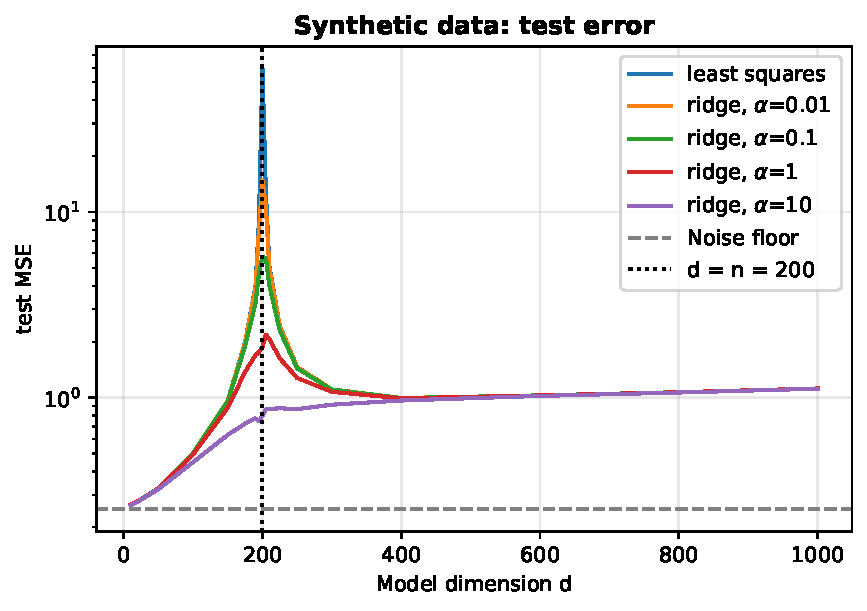
\includegraphics[width=\textwidth]{figures/synthetic_test.pdf}
    \caption{Test MSE vs.\ model dimension $d$.}
    \label{fig:syn_test}
  \end{subfigure}
  \hfill
  \begin{subfigure}[b]{0.49\textwidth}
    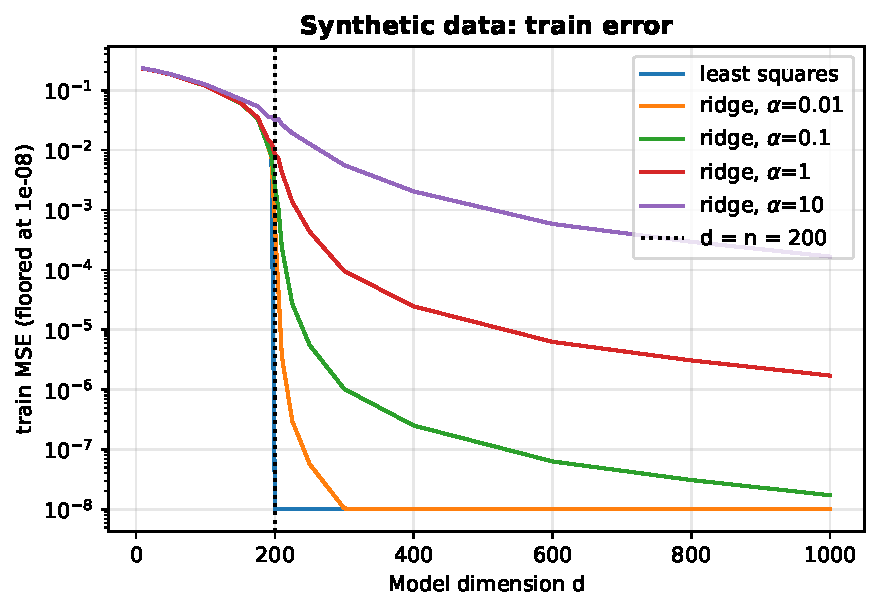
\includegraphics[width=\textwidth]{figures/synthetic_train.pdf}
    \caption{Train MSE vs.\ model dimension $d$.}
    \label{fig:syn_train}
  \end{subfigure}
  \caption{Synthetic dataset: least squares and ridge regression.
           The vertical dotted line marks the interpolation threshold $d = n = 200$.
           The horizontal dashed line marks the noise floor $\sigma^2 = 0.25$.}
  \label{fig:synthetic}
\end{figure}

\paragraph{Double descent.}
Figure~\ref{fig:syn_test} clearly shows double descent for OLS (``least squares'').
In the under-parametrised regime ($d < 200$), the test error decreases as $d$ grows and the
model acquires more expressive power.
At $d = n = 200$ there is a sharp spike: the interpolation threshold.
In the over-parametrised regime ($d > 200$), the test error decreases monotonically,
approaching the noise floor $\sigma^2 = 0.25$.

\paragraph{Training error.}
Figure~\ref{fig:syn_train} confirms the expected behaviour.
For $d < n$, OLS leaves a non-zero training residual; the error decreases with $d$ as the
model gains capacity.
At $d = n$, training error drops to machine precision (the system is exactly determined).
For $d > n$, training error stays at (numerical) zero since the minimum-norm interpolant
perfectly fits all training points by construction.

\paragraph{Ridge regression.}
Ridge regression eliminates the interpolation spike for all tested $\lambda$ values.
The regularisation penalty shrinks the weight vector and prevents the catastrophic
amplification of noise that occurs when $X^\top X$ is nearly singular.
For strong regularisation ($\lambda = 10$), the test error is controlled throughout but
remains above the noise floor even for large $d$, reflecting the bias introduced by
excessive shrinkage.
For weak regularisation ($\lambda = 0.01$), the curve closely tracks OLS in the
under-parametrised regime and smooths the spike, giving the best of both worlds.

\begin{figure}[H]
  \centering
  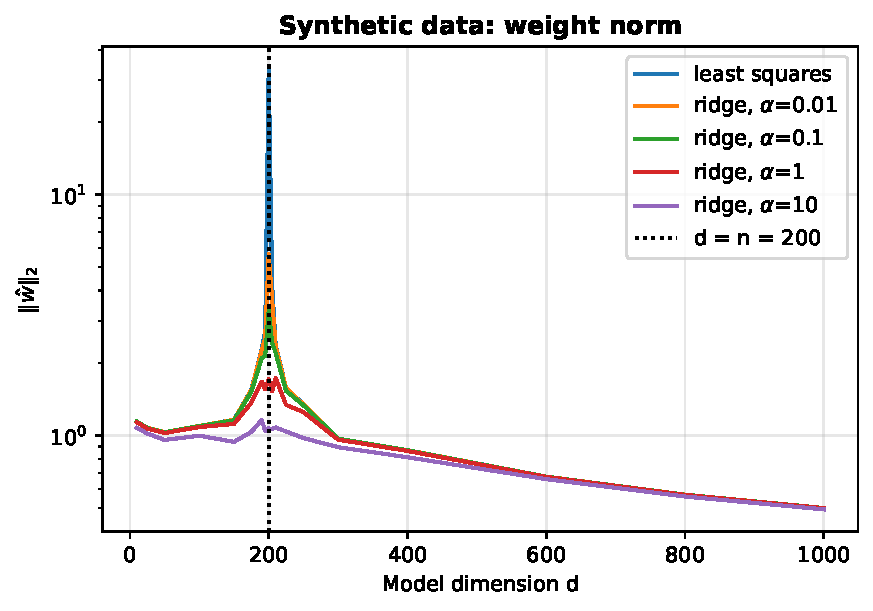
\includegraphics[width=0.55\textwidth]{figures/synthetic_weight_norm.pdf}
  \caption{Synthetic dataset: $\ell_2$ norm of the fitted weight vector $\|\hat{w}\|_2$.}
  \label{fig:syn_norm}
\end{figure}

\paragraph{Weight norm.}
Figure~\ref{fig:syn_norm} illustrates why the interpolation threshold is so dangerous for OLS.
Near $d = n$, $\|\hat{w}\|_2$ spikes dramatically: the near-singular normal equations force
the solver to use enormous coefficient values to interpolate the data, which amplify noise on
the test set.
For $d \gg n$, the minimum-norm constraint suppresses $\|\hat{w}\|_2$, and the estimator
reverts to a well-behaved solution.
Ridge regression keeps $\|\hat{w}\|_2$ uniformly bounded by design, explaining the absence
of the spike.

\subsection{Real-World Data: California Housing}

\begin{figure}[H]
  \centering
  \begin{subfigure}[b]{0.49\textwidth}
    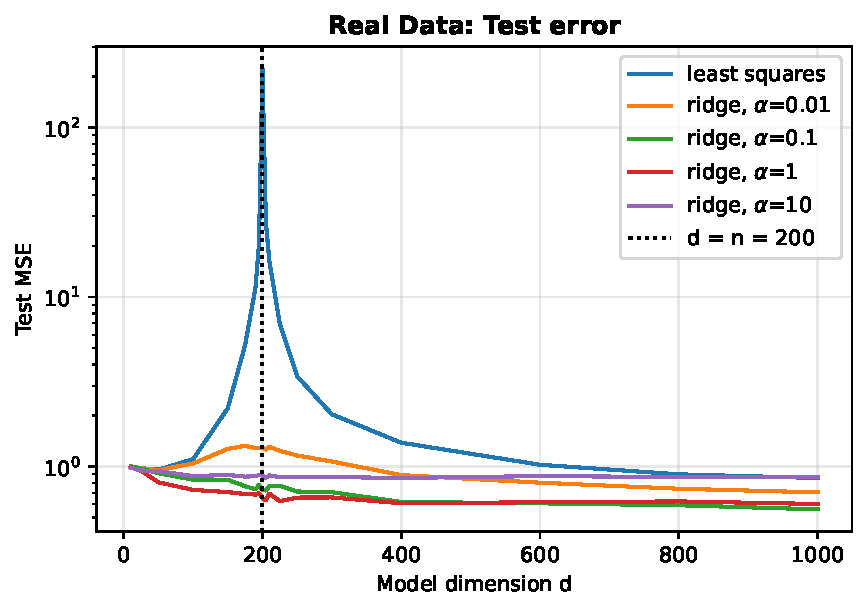
\includegraphics[width=\textwidth]{figures/real_test.pdf}
    \caption{Test MSE vs.\ model dimension $d$.}
    \label{fig:real_test}
  \end{subfigure}
  \hfill
  \begin{subfigure}[b]{0.49\textwidth}
    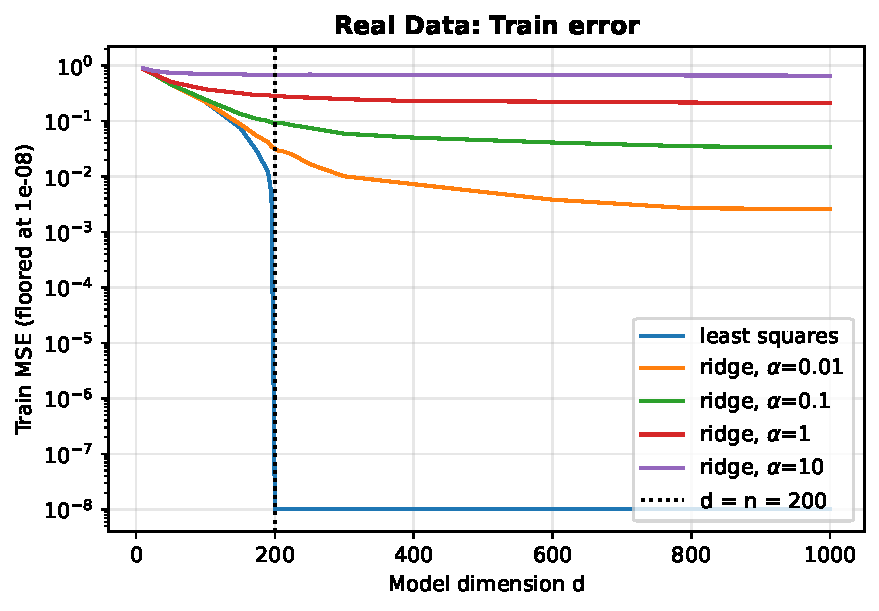
\includegraphics[width=\textwidth]{figures/real_train.pdf}
    \caption{Train MSE vs.\ model dimension $d$.}
    \label{fig:real_train}
  \end{subfigure}
  \caption{Real dataset (California Housing with random Fourier features).
           The vertical dotted line marks $d = n = 200$.}
  \label{fig:real}
\end{figure}

\paragraph{Qualitative agreement.}
Figure~\ref{fig:real_test} shows that double descent is also visible on the real dataset,
confirming that the phenomenon is not limited to synthetic settings.
The spike at $d = n$ is less sharp than in the synthetic case due to the additional noise
sources inherent in real data (label noise, model misspecification), but it is clearly present.

\paragraph{Differences from the synthetic case.}
In the over-parametrised regime, the OLS test error does not drop below the level achieved in
the best under-parametrised regime, as it does for the synthetic case.
This is because the RBF kernel representation introduces approximation error (the true
relationship between features and house values is not linear in the RFF embedding), and
increasing $d$ cannot remove this structural mismatch.
As a result, the second descent is shallower, and there is a range of $d$ values where
neither the under- nor the over-parametrised model generalises well.

\paragraph{Ridge regression.}
As with the synthetic data, ridge regression eliminates the spike and achieves consistently
lower test error across all $d$ values.
The optimal regularisation strength ($\lambda \approx 0.1$--$1$) leads to a test error that
is monotonically decreasing, closely tracking the lower envelope of the OLS curve.

\begin{figure}[H]
  \centering
  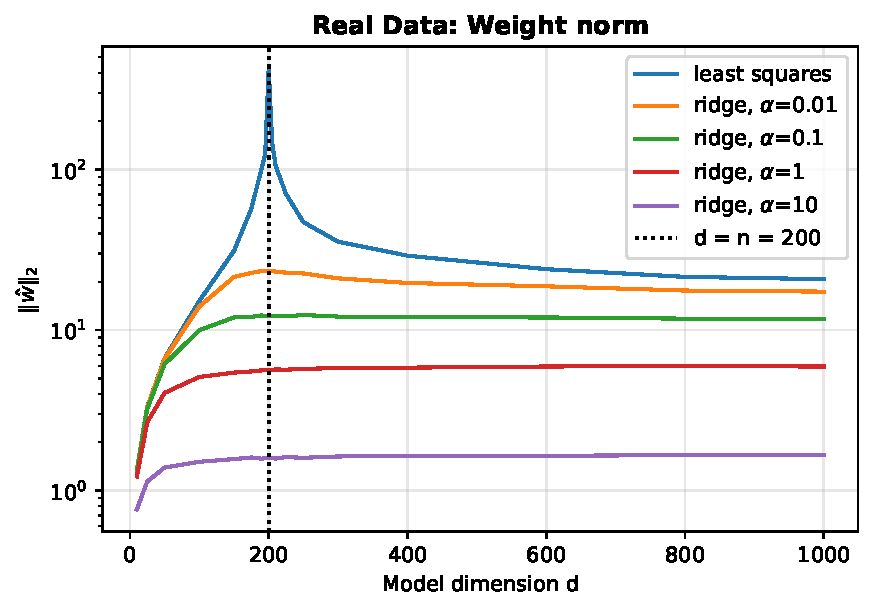
\includegraphics[width=0.55\textwidth]{figures/real_weight_norm.pdf}
  \caption{Real dataset: $\ell_2$ norm of the fitted weight vector.}
  \label{fig:real_norm}
\end{figure}

Figure~\ref{fig:real_norm} mirrors the synthetic weight norm plot: OLS exhibits a sharp
spike in $\|\hat{w}\|_2$ at $d = n$, while ridge regression keeps it bounded.


% ============================================================
\section{Extensions}
\label{sec:extensions}
% ============================================================

\subsection{Effect of Noise}

\begin{figure}[H]
  \centering
  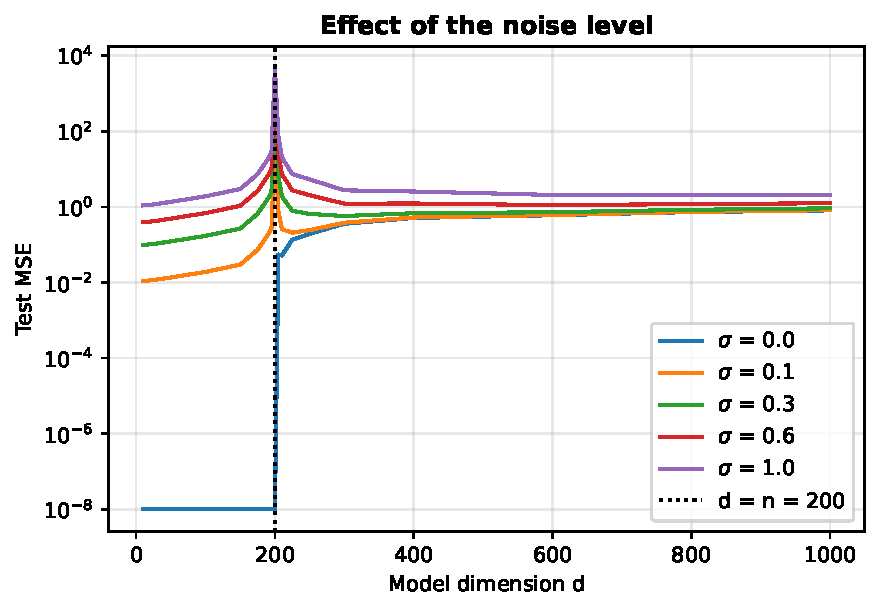
\includegraphics[width=0.6\textwidth]{figures/noise_effect.pdf}
  \caption{Effect of the noise level $\sigma$ on the test MSE of OLS.
           Each curve corresponds to a different noise standard deviation.}
  \label{fig:noise}
\end{figure}

Figure~\ref{fig:noise} shows the OLS test MSE for five noise levels
$\sigma \in \{0.0, 0.1, 0.3, 0.6, 1.0\}$.

\paragraph{Key observations.}
\begin{enumerate}
  \item \textbf{Noise-free case ($\sigma = 0$):} there is \emph{no} double descent.
        For $d < n$ the model simply fails to express the true $\beta^*$ exactly (bias), and
        the error monotonically decreases to zero once $d \ge n$.
        The interpolation threshold causes no spike because there is no noise to amplify.
  \item \textbf{Low noise ($\sigma = 0.1$):} a mild spike appears at $d = n$, and the
        over-parametrised error quickly drops below the under-parametrised optimum.
  \item \textbf{High noise ($\sigma = 1.0$):} the spike is much larger, and the second
        descent is slower; the over-parametrised error approaches a higher noise floor
        ($\sigma^2 = 1.0$).
\end{enumerate}

This confirms that the double descent spike is a \emph{noise amplification} effect: the
minimum-norm interpolant is forced to fit the noisy training labels, amplifying the noise
when the normal equations are nearly singular.
In the noiseless limit, double descent vanishes.

\subsection{Bias--Variance Decomposition}

\begin{figure}[H]
  \centering
  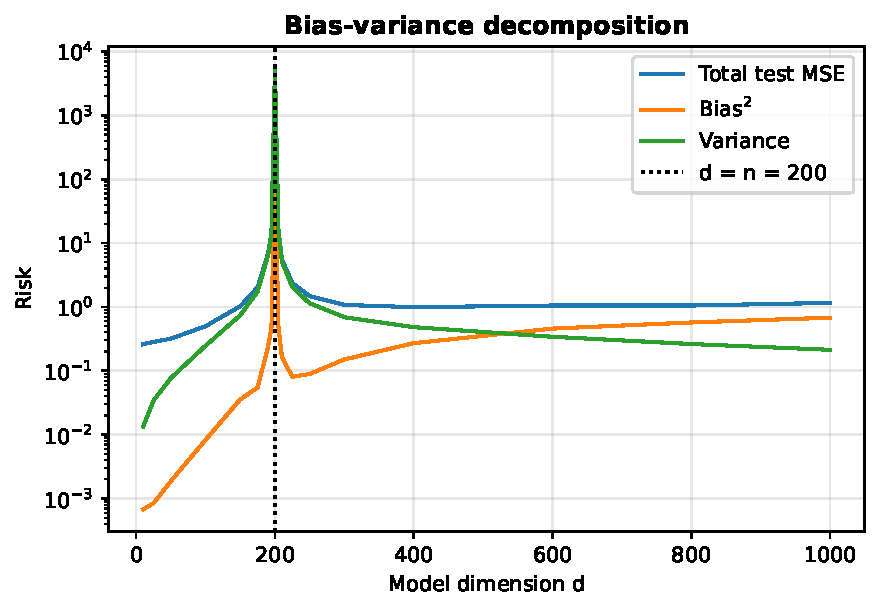
\includegraphics[width=0.6\textwidth]{figures/bias_variance.pdf}
  \caption{Bias--variance decomposition of the OLS test risk (synthetic data, $\sigma = 0.5$).}
  \label{fig:bv}
\end{figure}

Figure~\ref{fig:bv} plots the empirical bias$^2$, variance, and total test MSE of OLS as
functions of $d$.

\paragraph{Classical regime ($d < n$).}
Both bias and variance contribute.
Bias decreases with $d$ as the model gains expressive power.
Variance is moderate and roughly flat.
The total risk is dominated by bias and falls monotonically.

\paragraph{At the interpolation threshold ($d \approx n$).}
Variance explodes as the normal equations become ill-conditioned.
Bias is close to zero (the model is nearly expressive enough to represent $\beta^*$ exactly),
but variance overwhelms this benefit, causing the total risk to spike.

\paragraph{Over-parametrised regime ($d > n$).}
Variance decreases monotonically and eventually falls below $\sigma^2$.
Bias decreases as well (the minimum-norm solution in a larger space is a better approximation
of $\beta^*$ when projected onto the test distribution).
The total risk converges to $\sigma^2 = 0.25$ from above.

This decomposition provides a precise picture of the classical claim that the
bias--variance trade-off implies a single optimal complexity: the claim only holds in the
classical regime.
In the over-parametrised regime, \emph{both} bias and variance can decrease simultaneously,
breaking the alleged trade-off.


% ============================================================
\section{Discussion}
\label{sec:discussion}
% ============================================================

\subsection{Positive Aspects}

\begin{itemize}
  \item \textbf{Clean empirical reproduction.}
        Both datasets exhibit the double descent phenomenon clearly.
        The synthetic experiment reproduces all qualitative features predicted by theory:
        monotone decrease in the classical regime, spike at $d = n$, and monotone recovery
        in the over-parametrised regime.

  \item \textbf{Ridge mitigates the spike.}
        Ridge regression provides a robust alternative to OLS across all $d$ values.
        Even a small regularisation parameter ($\lambda = 0.01$) eliminates the interpolation
        spike without incurring significant bias.

  \item \textbf{Bias--variance decomposition is instructive.}
        Empirically decomposing bias and variance confirms the theoretical prediction that the
        spike is entirely driven by a variance explosion, and that the second descent is driven
        by variance reduction rather than bias increase.

  \item \textbf{Noise analysis.}
        Varying $\sigma$ cleanly demonstrates that the spike disappears in the noiseless limit
        and grows proportionally to the noise level, providing a complete qualitative picture
        of when double descent matters in practice.
\end{itemize}

\subsection{Limitations and Negative Aspects}

\begin{itemize}
  \item \textbf{Finite $T$ approximation.}
        With only $T = 30$ trials, the median near $d = n$ may not fully capture the
        true spike height; the variance of the spike estimator is high in that region.
        A larger number of trials would provide smoother and more reliable estimates.

  \item \textbf{Approximation quality of RFF.}
        The random Fourier feature approximation of the RBF kernel introduces additional
        randomness.
        In our setup, each trial $t$ uses a new random RFF matrix $W$ (tied to the same
        seed as the data split), so the RFF approximation error is part of the variance
        reported.
        Fixing $W$ across trials would separate approximation error from sampling variance.

  \item \textbf{Shallow second descent on real data.}
        On California Housing, the second descent is less pronounced than on synthetic data.
        The true relationship between census features and house prices is non-linear, so
        RFF-expanded linear regression is a misspecified model.
        The remaining approximation error sets a floor on how much the second descent can help.

  \item \textbf{Small $n_{\mathrm{train}}$.}
        Using only $n = 200$ training samples (out of $20{,}640$ available) is intentional
        for exhibiting double descent at moderate $d$, but it limits the absolute quality of
        predictions and may not be representative of real-world deployment conditions.

  \item \textbf{No gradient descent extension.}
        The assignment extension mentions gradient descent vs.\ closed-form.
        We focus here on closed-form solutions, which are exact; adding gradient descent would
        allow studying how implicit regularisation of gradient descent interacts with the
        double descent phenomenon (see \cite{ali2019continuous}).
\end{itemize}


% ============================================================
\section{Conclusion}
\label{sec:conclusion}
% ============================================================

We have empirically reproduced the double descent risk curve of Belkin et al.\ \cite{belkin2019reconciling}
for linear regression.
Fixing $n = 200$ and sweeping the model dimension $d$ from 10 to 1000, we observe:

\begin{enumerate}
  \item A classical bias--variance trade-off curve for $d < n$, with test error decreasing as
        the model gains capacity.
  \item A sharp spike at the interpolation threshold $d = n = 200$, caused by the ill-conditioning
        of $X^\top X$ and the resulting explosion of variance.
  \item A monotone second descent for $d > n$, where the minimum-norm interpolant's variance
        decreases as the model dimension grows.
\end{enumerate}

Ridge regression eliminates the spike by ensuring the normal equations remain well-conditioned.
Noise analysis confirms that the spike is a noise amplification phenomenon absent in the
noiseless case.
The bias--variance decomposition shows that the second descent involves simultaneous reduction
of both bias and variance, challenging the classical intuition that these two quantities must
trade off.

\bigskip
\noindent
\textbf{Code availability.}
All code is available in the repository at \url{https://github.com/student/double-descent-linear}.
Figures are generated by running \texttt{python experiments.py}.

% ============================================================
\begin{thebibliography}{9}

\bibitem{belkin2019reconciling}
M.~Belkin, D.~Hsu, S.~Ma, and S.~Mandal.
\newblock Reconciling modern machine learning practice and the classical bias--variance trade-off.
\newblock \emph{Proceedings of the National Academy of Sciences}, 116(32):15849--15854, 2019.

\bibitem{bartlett2020benign}
P.~L.~Bartlett, P.~M.~Long, G.~Lugosi, and A.~Tsigler.
\newblock Benign overfitting in linear regression.
\newblock \emph{Proceedings of the National Academy of Sciences}, 117(48):30063--30070, 2020.

\bibitem{pace1997sparse}
R.~K.~Pace and R.~Barry.
\newblock Sparse spatial autoregressions.
\newblock \emph{Statistics \& Probability Letters}, 33(3):291--297, 1997.

\bibitem{rahimi2007random}
A.~Rahimi and B.~Recht.
\newblock Random features for large-scale kernel machines.
\newblock In \emph{Advances in Neural Information Processing Systems (NeurIPS)}, volume 20, 2007.

\bibitem{ali2019continuous}
A.~Ali, E.~Dobriban, and R.~J.~Tibshirani.
\newblock The implicit regularization of stochastic gradient flow for least squares.
\newblock In \emph{Proceedings of the 37th International Conference on Machine Learning (ICML)}, 2020.

\end{thebibliography}

\end{document}
